%Include simulation results: both wave forms in time domain, and in frequency domain (apply FFT) (assignments 3 and 4 only).
Figure~\ref{fig:simulation:waveform} shows a comparison of the waveform for the input and the output audio.
As is shown here, these images are very similar.
This gives us a first indication that the output is indeed a resampled version of the input.
As shown on the left, the input has a sample rate of 44100Hz, while the output has a sample rate of 48000Hz.

\begin{figure}[H]
	\centering
	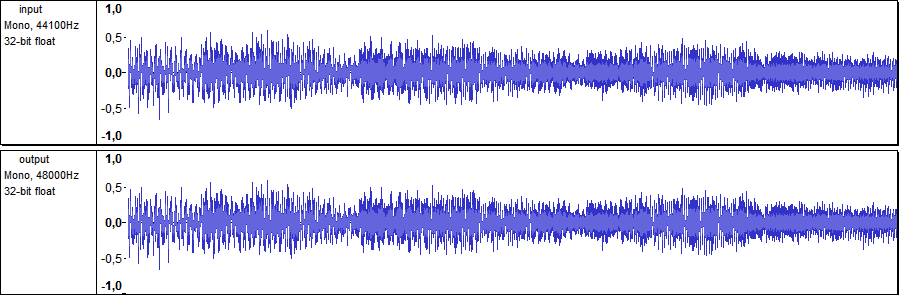
\includegraphics[width=0.9\textwidth]{comparison}
	\caption{Comparison of the waveform for the input and the output}
	\label{fig:simulation:waveform}
\end{figure}

If we zoom in a bit further, as can be seen in Figure~\ref{fig:simulation:waveformzoom}, the waveform of the input and the waveform of the output are still very similar.

\begin{figure}[H]
	\centering
	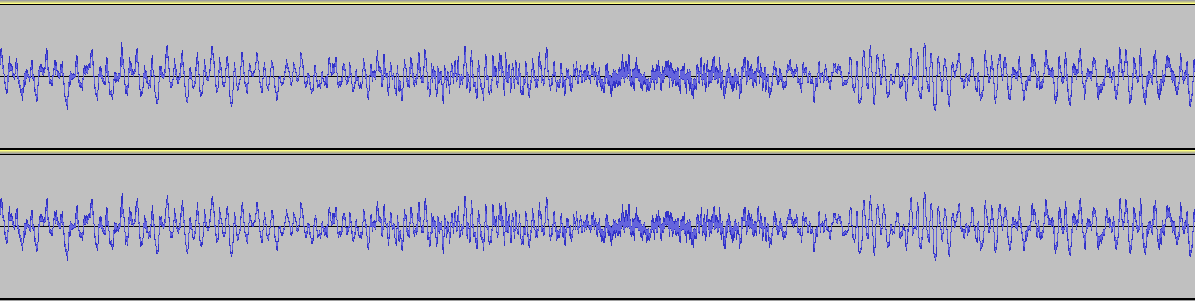
\includegraphics[width=0.9\textwidth]{comparison-zoom}
	\caption{Comparison of the waveform for the input and the output, zoomed in slightly}
	\label{fig:simulation:waveformzoom}
\end{figure}

Figure~\ref{fig:simulation:spectrum} shows the spectrum analysis of the input and the output files.
We can see that up to about 18kHz, the frequency analysis looks very much alike.
After that point, the input and output start to differ.
However, the instructor has assured us that this difference is negligible.

\begin{figure}[H]
	\centering
	\begin{subfigure}[l]{0.7\textwidth}
		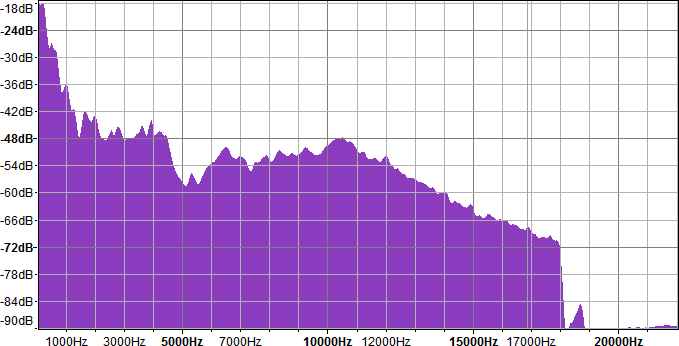
\includegraphics[width=\textwidth]{freq-input}
		\caption{Input}
		\label{fig:simulation:spectrum:before}
	\end{subfigure}

	\begin{subfigure}[l]{0.7\textwidth}
		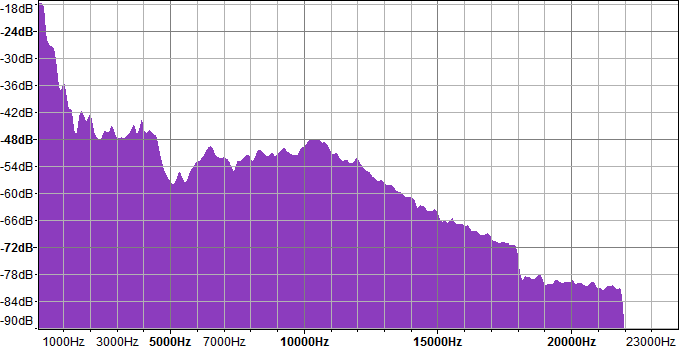
\includegraphics[width=\textwidth]{freq-output}
		\caption{Output}
		\label{fig:simulation:spectrum:after}
	\end{subfigure}

	\caption{Comparison of the audio spectrum before and after running the filter}
	\label{fig:simulation:spectrum}
\end{figure}

When we simulated our design with a stream index of anything other than 0, we got some weird results.
Figure~\ref{fig:simulation:spectrum:wrong} gives the spectrum analysis of one of the streams in the output.
The problem is related to the way we initialize the coefficients.
After some investigation, we found that there were always two streams that were completely correct.
The rest of the streams all exhibit this behaviour (though the number of streams does not seem to impact the severity of the errors).
We can shift which two streams are correct by modifying some parameters, but we were not able to solve the problem entirely.

\begin{figure}[H]
	\centering
	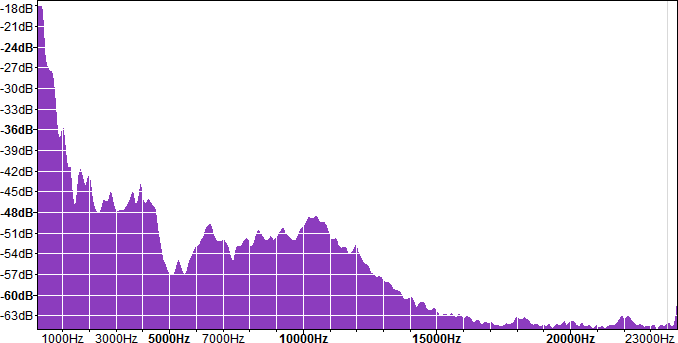
\includegraphics[width=0.9\textwidth]{freq-wrong}
	\caption{Spectrum analysis for stream with non-zero index}
	\label{fig:simulation:spectrum:wrong}
\end{figure}

We expect that there are just some garbage values in the output.
As we can see when we compare Figure~\ref{fig:simulation:spectrum:wrong} to Figure~\ref{fig:simulation:spectrum:after}, most of the spectrum is actually the same.
It is only above 18kHz that the spectrum analyses begin to differ.
In some other cases, we have seen weird values below 1kHz too.
The audio does sound the same.
